%% This work is distributed under the LaTeX Project Public License (LPPL)
%% ( http://www.latex-project.org/ ) version 1.3, and may be freely used,
%% distributed and modified. A copy of the LPPL, version 1.3, is included
%% in the base LaTeX documentation of all distributions of LaTeX released
%% 2003/12/01 or later.
%% Retain all contribution notices and credits.
%% ** Modified files should be clearly indicated as such, including  **
%% ** renaming them and changing author support contact information. **
%%*************************************************************************
\documentclass[conference]{IEEEtran}
\usepackage{fontspec}
\setmainfont[
 Path = ./ ,
 Extension = .otf ,
 Mapping=tex-text,
 Ligatures={TeX, Common},
 BoldFont = texgyretermes-bold,
 ItalicFont = texgyretermes-italic,
 BoldItalicFont = texgyretermes-bolditalic,
 SmallCapsFont = texgyretermes,
 SmallCapsFeatures = {Letters = SmallCaps}
]{texgyretermes}

\usepackage{polyglossia}
\setdefaultlanguage{english}
% \setotherlanguages{english}

\usepackage[backend=biber,style=ieee,refsection=section]{biblatex}    
% *** CITATION PACKAGES ***
%
% \usepackage{cite}
% cite.sty was written by Donald Arseneau
% V1.6 and later of IEEEtran pre-defines the format of the cite.sty package
% \cite{} output to follow that of the IEEE. Loading the cite package will
% result in citation numbers being automatically sorted and properly
% "compressed/ranged". e.g., [1], [9], [2], [7], [5], [6] without using
% cite.sty will become [1], [2], [5]--[7], [9] using cite.sty. cite.sty's
% \cite will automatically add leading space, if needed. Use cite.sty's
% noadjust option (cite.sty V3.8 and later) if you want to turn this off
% such as if a citation ever needs to be enclosed in parenthesis.
% cite.sty is already installed on most LaTeX systems. Be sure and use
% version 5.0 (2009-03-20) and later if using hyperref.sty.
% The latest version can be obtained at:
% http://www.ctan.org/pkg/cite
% The documentation is contained in the cite.sty file itself.

\usepackage{graphicx}
\usepackage{amsmath}
\usepackage{url}
\usepackage{array}
\usepackage[caption=false,font=footnotesize]{subfig}
\usepackage{lipsum}
% \usepackage[caption=false,font=footnotesize]{subfig}
% \usepackage{dblfloatfix}
% The latest version can be found at:
% http://www.ctan.org/pkg/dblfloatfix

\renewcommand{\thesubsection}{\Alph{subsection}.}
\renewcommand{\thesubsubsection}{\arabic{subsubsection})}
\renewcommand{\theparagraph}{\alph{paragraph})}


% The following code makes "fake small caps" which work fine
% for cyrillic symbols
% Borrowed from http://tex.stackexchange.com/questions/64582/faking-small-caps-in-xelatex?rq=1


\usepackage{expl3,xparse}

% turn expl3 space on: `:' and `_' are letters now and spaces
% are ignored. To insert a space use `~'.
\ExplSyntaxOn
% the internal command:
\cs_new:Npn \fakecaps:n #1
  {
    \addfontfeature{LetterSpace=10.0} {\tl_head:n { #1 }\kern 1pt}{\addfontfeature{Scale=0.9}\uppercase{\tl_tail:n { #1 }}}
  }

% the document command:
\NewDocumentCommand\FakeCaps{m}
  {\fakecaps:n { #1 } }

% turn expl3 space off again:
\ExplSyntaxOff

\makeatletter
\newcommand\subparagraph{%
  \@startsection{subparagraph}{5}
  {\parindent}
  {3.25ex \@plus 1ex \@minus .2ex}
  {-1em}
  {\normalfont\normalsize\bfseries}}
\makeatother
\usepackage[explicit]{titlesec}
\let\subparagraph\relax
\titleformat{\section}[hang]{\normalfont\normalsize\centering}{\thesection.}{0.5em}{\FakeCaps{#1}}

\makeatletter
\def\russian@capsformat{}
\makeatother


%% Bibliography file
\addbibresource{seim.bib}


% If you need to correct hyphenations, add them here
\hyphenation{op-tical net-works semi-conduc-tor}


\begin{document}
%
% paper title
%
% In English titles are generally capitalized except for words such as a, an, and, as,
% at, but, by, for, in, nor, of, on, or, the, to and up, which are usually
% not capitalized unless they are the first or last word of the title.
% Linebreaks \\ can be used within to get better formatting as desired.
% Do not put math or special symbols in the title.
\title{Effectively Compressing Embedded GNU/Linux \\ and Windows 10 IoT Images Using XZ}


% author names and affiliations
% use a multiple column layout for up to three different
% affiliations
\author{\IEEEauthorblockN{Roman Belkov}
\IEEEauthorblockA{Saint Petersburg State University\\
Email: roman.belkov@gmail.com}
\and
\IEEEauthorblockN{Iakov Kirilenko}
\IEEEauthorblockA{Saint Petersburg State University\\
Email: y.kirilenko@spbu.ru}
}

% make the title area
\maketitle

% As a general rule, do not put math, special symbols or citations
% in the abstract
\begin{abstract}Nowadays, Internet of Things is very popular and it has a lot of software that has to be distributed to users over the Internet. Since storage space and bandwidth are limited, data compression becomes crucial. However, often outdated or improperly set up tools are used for compression due to the neglecting of the matter at hand. An attempt to achieve better compression ratio for Internet of Things devices' firmware using the iterative experiment over the options that XZ Utils has to offer is presented. Authors tried to analyze if accurate tuning of options in addition to application of a proper tool will have a positive impact on the situation and improve current compression ratios. As a result of work, improvement in compression ratio by up to 35\% is presented when compared to the initial compressed images.
% * <Максим Голов> 14:16:34 17 Mar 2016 UTC+0300:
% 1) Since storage space and bandwidth are limited, data compression becomes crucial.
% 2) However, often outdated or improperly set up tools are used for compression due to the neglecting of the matter at hand.
% 3) Authors tried to see if accurate tuning of options in addition to application of a proper tool will have an impact on the situation and improve current compression ratios.
% 4) As a result, authors were able to improve compression ratio by up to 35%.
\end{abstract}

\section{Introduction}
% no \IEEEPARstart

Despite rapid growth in storage space and Internet connection bandwidth, demand for bigger storage and better transfer speed rise even faster, not to mention that available technology varies drastically in different regions. Data compression is the thing that can save the world precious time and limited storage. Data compression can be achieved by various techniques and for different purposes, but in this paper we focus on compressing firmware images for Internet of Things devices. IoT's popularity has sky-rocketed over the past five years, which resulted in creation of a lot of sotware that takes up a a lot of space on servers and takes some time to transfer over the networks. 
% * <Максим Голов> 14:22:48 17 Mar 2016 UTC+0300:
% 1) Despite rapid growth in storage space and Internet bandwidth, demand for bigger storage and better transfer speed rise even faster, not to mention that available technology varies drastically in different regions.
% 2) IoT's popularity has sky-rocketed over the past five years, which resulted in creation of a lot of sotware that takes up a a lot of space on servers and takes some time to transfer over the networks.

The goal of this research is to try and optimize the compression of firmware images in case of distributing the images. Basically, we want to compress only once and after that archive will only be downloaded from servers and extracted by users. That makes minimization of compressed image's size our top priority. Because usually image is compressed on the same computer that was used to build a firmware image (which makes this computer quite powerful), it is safe to assure that this machine has all the needed resources and is capable of compressing the output image quite fast (comparing to build time, of course).
% * <Максим Голов> 14:25:41 17 Mar 2016 UTC+0300:
% 1) The goal of this research is to try and optimize the compression of firmware images in case of distributing the images.

Authors have chosen XZ Utils as the tool for the experiment, because today it is one of the most powerful compression tools, which is widely used by the community even in large-scale projects \cite{link:fedora-xz} \cite{link:kernel-xz}.
% * <Максим Голов> 14:27:59 17 Mar 2016 UTC+0300:
% 1) Authors have chosen XZ Utils as the tool for the experiment, because today it is one of the most powerful compression tools, which is widely used by the community even in large-scale projects

\section{Experiment}
\label{sec:experiment}

\subsection{Description}

For experiment, we have chosen four different images for four different controllers:
\begin{itemize}
\item TRIK firmware -- ARM architecture
\item Raspbian      -- ARM architecture
\item Raspberry Pi Windows 10 IoT -- ARM architecture
\item MinnowBoard Max Windows 10 IoT -- x86 architecture
\end{itemize}

We used XZ utils 5.2.1 on a Fedora 23-driven local PC and XZ utils 5.2.1 on two Azure VM that ran Ubuntu 14.04 LTS. Necessity in Azure VM appeared when we wanted to see results of running XZ with dictionary sizes of 1024 and 1536 megabytes, while local PC allowed us to go no more than 512 megabytes, since it had only 8GB of RAM.
% * <Максим Голов> 14:30:22 17 Mar 2016 UTC+0300:
% 1) Necessity in Azure VM appeared when we wanted to see results of running XZ (надо капс?) with dictionary sizes of 1024 and 1536 megabytes, while local PC allowed us to go no more than 512 megabytes, since it had only 8GB of RAM.


\subsection{Big Dictionaries}

% An example of a floating figure using the graphicx package.
% Note that \label must occur AFTER (or within) \caption.
% For figures, \caption should occur after the \includegraphics.
% Note that IEEEtran v1.7 and later has special internal code that
% is designed to preserve the operation of \label within \caption
% even when the captionsoff option is in effect. However, because
% of issues like this, it may be the safest practice to put all your
% \label just after \caption rather than within \caption{}.
%
% Reminder: the "draftcls" or "draftclsnofoot", not "draft", class
% option should be used if it is desired that the figures are to be
% displayed while in draft mode.
%
% \begin{figure}[!t]
% \centering
% 
\includegraphics[width=2.5in]{latex.pdf}
% \caption{Simulation results for the network.}
% \label{fig_sim}
% \end{figure}

% \subsubsection{Subsubsection Heading Here}

% Note that the IEEE typically puts floats only at the top, even when this
% results in a large percentage of a column being occupied by floats.

% An example of a double column floating figure using two subfigures.
% (The subfig.sty package must be loaded for this to work.)
% The subfigure \label commands are set within each subfloat command,
% and the \label for the overall figure must come after \caption.
% \hfil is used as a separator to get equal spacing.
% Watch out that the combined width of all the subfigures on a 
% line do not exceed the text width or a line break will occur.
%
% \begin{figure*}[!t]
% \centering
% \subfloat[Case I]{
\includegraphics[width=2.5in]{latex.pdf}%
% \label{fig_first_case}}
% \hfil
% \subfloat[Case II]{
\includegraphics[width=2.5in]{latex.pdf}%
% \label{fig_second_case}}
% \caption{Simulation results for the network.}
% \label{fig_sim}
% \end{figure*}

% \lipsum[1-4]

We started by measuring compression rates using default XZ presets. The set of presets is divided into two major subsets: standard (from 0 to 9) and extreme (from 0e to 9e). In theory, using extreme presets results in better compression ratio since they provide a set of options for LZMA2 algorithm that should give better compression ratios, but in reality for our images 8 and 8e / 9 and 9e gave the same results, so for now we will not differentiate them.
% * <Максим Голов> 14:35:41 17 Mar 2016 UTC+0300:
% 1) We started by measuring compression rates using default XZ presets.
% 2) In theory, using extreme presets results in better compression ratio since they yield a set of options for LZMA2 algorithm that should give better compression ratio, but on practice for our images 8 and 8e / 9 and 9e gave the same results, so for now we will not differentiate them.
% ^ <Максим Голов> 14:52:29 17 Mar 2016 UTC+0300:
% Лучше вариант
% 2) In theory, using extreme presets results in better compression ratio since they provide a set of options for LZMA2 algorithm that should give better compression ratios, but in reality for our images 8 and 8e / 9 and 9e gave the same results, so for now we will not differentiate them.

Remarkably, using standard presets from 6 to 9 gives the same set of options for LZMA2 algorithm except the dictionary size setting. Since preset 9 results in 64MB dictionary and the maximum value for dictionary is 1536MB, we decided to see what will happen with an increase in dictionary size.
% * <Максим Голов> 14:38:02 17 Mar 2016 UTC+0300:
% 1) Remarkably, using standard presets from 6 to 9 gives the same set of options for LZMA2 algorithm except the dictionary size setting. Since preset 9 results in 64MB dictionary and the maximum value for dictionary is 1536MB, we decided to see what will happen with an increase in dictionary size.

\begin{table}[h]
\renewcommand{\arraystretch}{1.5}
% if using array.sty, it might be a good idea to tweak the value of
% \extrarowheight as needed to properly center the text within the cells
\caption{Big dictionaries}
\label{big_dictionary_table}
\centering
\begin{tabular}{| l *{4}{| c } |}
    \hline
    Dictionary & TRIK & Raspbian & RPi Win10 & MB Win10 \\
    \hline
    128 & 0,85 & 0,75 & 1,25 & 0,97 \\
    256 & 2,71 & 1,06 & 2,43 & 2,09 \\
    512 & 3,18 & 1,52 & 4,16 & 4,16 \\
    1024 & 3,26 & 2,01 & 4,69 & 5,06 \\
    1536 & 3,26 & 2,92 & 4,69 & 5,08 \\
\hline
\end{tabular}
\end{table}

As can be seen in Table \ref{big_dictionary_table}, we improved the compression ratio over standard XZ 9 preset, especially when compressing Windows 10 IoT images.
% * <Максим Голов> 14:41:31 17 Mar 2016 UTC+0300:
% Тут не уверен, но если "улучшили производительность", то лучше "we improved the performance"
% "xz -9" -- тут, возможно капс (XZ) и если говоришь о пресетах, то напиши, что это пресет. я не понимаю, о чем это


\subsection{BCJ Filters}
\label{subsec:bcj}

XZ offers users a Branch-Call-Jump filter that is specifically designed for compressing binaries. BCJ filter converts relative addresses in the machine code to their absolute counterparts. This does not change the size of the data, but it increases redundancy, which can help LZMA2 produce 0-15\% smaller .xz file. \cite{link:xz-specs}
% * <Максим Голов> 14:50:48 17 Mar 2016 UTC+0300:
% 1) XZ offers users a Branch-Call-Jump filter that is specifically designed for compressing binaries.
% 2) This doesn't change the size of the data, but it increases redundancy, which can help LZMA2 produce up to 15\% smaller .xz file.

At this stage we encouter the following problem: the firmware image is not one entire binary file, so in theory blindly applying BCJ filter is not a good idea, but we decided to go on and see what happens. Minding the theory, though, we must note that a whole lot of possibilities lies here, because there may be some ways to compress parts of firmware independently that can possibly result in a better compression ratio.
% * <Максим Голов> 14:55:44 17 Mar 2016 UTC+0300:
% 1) At this stage we encouter the following problem: the firmware image is not one entire binary file, so in theory blindly applying BCJ filter is not a good idea, but we decided to go on and see what happens. 
% 2) Minding the theory, though, we must note that a whole lot of possibilities lies here, because there may be some ways to compress parts of firmware independently that can possibly result in a better compression ratio.

\begin{table}[h]
\renewcommand{\arraystretch}{1.5}
% if using array.sty, it might be a good idea to tweak the value of
% \extrarowheight as needed to properly center the text within the cells
\caption{BCJ filters}
\label{bcj_table}
\centering
\begin{tabular}{| l *{4}{| c } |}
    \hline
    Dictionary & TRIK & Raspbian & RPi Win10 & MB Win10 \\
    \hline
    64 (pr. 9) & 2,56 & 1,56 & 2,59 & 3,47 \\
    128 & 2,56 & 2,31 & 3,71 & 4,32 \\
    256 & 4,96 & 2,61 & 4,89 & 5,41 \\
    512 & 5,51 & 3,06 & 6,59 & 7,36 \\
    1024 & 5,59 & 3,54 & 7,04 & 8,10 \\
    1536 & 5,59 & 4,43 & 7,04 & 8,20 \\
\hline
\end{tabular}
\end{table}

Results presented in the Table \ref{bcj_table} show improvement in compression ratios over standard XZ 9 preset in percent. One should note that dictionary size of 64 MB in this table is the result of applying BCJ filter to a XZ 9 preset.
% * <Максим Голов> 14:59:26 17 Mar 2016 UTC+0300:
% Забыл, что percent всегда в единственном числе -- поправь.
% * <Максим Голов> 14:58:16 17 Mar 2016 UTC+0300:
% 1) Results presented in the Table \ref{bcj_table} show improvement in compression ratios over standard xz -9 in percents.
% + посмотри капс на XZ и предыдущий коммент про "xz -9"

\subsection{Advanced Options}

After tweaking the dictionary size and BCJ filters, we decided to look into more advanced LZMA2 algorithm options and see what happens when we try to analyze compression results after randomizing those options. But before we announce the results, let us list the available options:
% * <Максим Голов> 15:02:01 17 Mar 2016 UTC+0300:
% 1) After tweaking the dictionary size and BCJ filters, we decided to look into more advanced LZMA2 algorithm options and see what happens when we try to analyze compression results after randomizing those options. But before we announce the results, let us list the available options:

\begin{itemize}
\item LC -- number of literal context bits 
\item LP -- number of literal position bits 
\item PB -- number of position bits 
\item Nice -- maximum match length 
% * <Максим Голов> 15:03:12 17 Mar 2016 UTC+0300:
% Тут точно "Nice"? Выглядит нелогично
\item Depth -- maximum search depth 
\end{itemize}

It is worth mentioning that LZMA2 filter also has following options: 

\begin{itemize}
\item Mode
\item MF -- match finder
\end{itemize}

In our research we decided to set Mode to 'normal' and MF to 'bt4' respectively as these are the settings that would give us maximum compression.

Analysis of the results gave us some pretty interesting facts. It turned out that compressing TRIK firmware image with dictionary size equal of 128 MB or 256 MB and with/without BCJ filter gives best result with the following setup:
% * <Максим Голов> 15:05:41 17 Mar 2016 UTC+0300:
% 1) Analysis of the results gave us some pretty interesting facts. It turned out that compressing TRIK firmware image with dictionary size of 128 MB or 256 MB and with/without BCJ filter gives best result with the following setup:
\begin{itemize}
\item lc=1
\item lp=2
\item pb=2
\item nice=192
\item depth=1024
\end{itemize}

%
% Note that often IEEE papers with subfigures do not employ subfigure
% captions (using the optional argument to \subfloat[]), but instead will
% reference/describe all of them (a), (b), etc., within the main caption.
% Be aware that for subfig.sty to generate the (a), (b), etc., subfigure
% labels, the optional argument to \subfloat must be present. If a
% subcaption is not desired, just leave its contents blank,
% e.g., \subfloat[].


% An example of a floating table. Note that, for IEEE style tables, the
% \caption command should come BEFORE the table and, given that table
% captions serve much like titles, are usually capitalized except for words
% such as a, an, and, as, at, but, by, for, in, nor, of, on, or, the, to
% and up, which are usually not capitalized unless they are the first or
% last word of the caption. Table text will default to \footnotesize as
% the IEEE normally uses this smaller font for tables.
% The \label must come after \caption as always.
%
% \begin{table}[!t]
% % increase table row spacing, adjust to taste
% \renewcommand{\arraystretch}{1.3}
% if using array.sty, it might be a good idea to tweak the value of
% \extrarowheight as needed to properly center the text within the cells
% \caption{An Example of a Table}
% \label{table_example}
% \centering
% % Some packages, such as MDW tools, offer better commands for making tables
% % than the plain LaTeX2e tabular which is used here.
% \begin{tabular}{|c||c|}
% \hline
% One & Two\\
% \hline
% Three & Four\\
% \hline
% \end{tabular}
% \end{table}

Table \ref{trik_improvements_table} and Figure \ref{trik_improvements_figure} shows improvement in compressing TRIK firmware image compared to standard XZ 9 preset setup:
% * <Максим Голов> 15:06:25 17 Mar 2016 UTC+0300:
% Тут опять может капс
% ^ <Максим Голов> 15:14:49 17 Mar 2016 UTC+0300:
% Лучше вариант
% Table \ref{trik_improvements_table} and Figure \ref{trik_improvements_figure} shows improvement in compressing TRIK firmware image compared to basic xz -9 setup:

\begin{table}[h]
\renewcommand{\arraystretch}{1.5}
% if using array.sty, it might be a good idea to tweak the value of
% \extrarowheight as needed to properly center the text within the cells
\caption{Improvements in compressing TRIK image}
\label{trik_improvements_table}
\centering
\begin{tabular}{| l *{3}{| c } |}
    \hline
    Dictionary & Default & ARM & Best + ARM \\
    \hline
    128 & 0,85 & 2,56 & 4,42 \\
    256 & 2,71 & 4,96 & 6,13 \\ 
    512 & 3,18 & 5,51 & 6,52 \\ 
    1024 & 3,26 & 5,59 & 6,67 \\ 
    1536 & 3,26 & 5,59 & 6,67 \\
\hline
\end{tabular}
\end{table}

\begin{figure}[h]
    \centering
	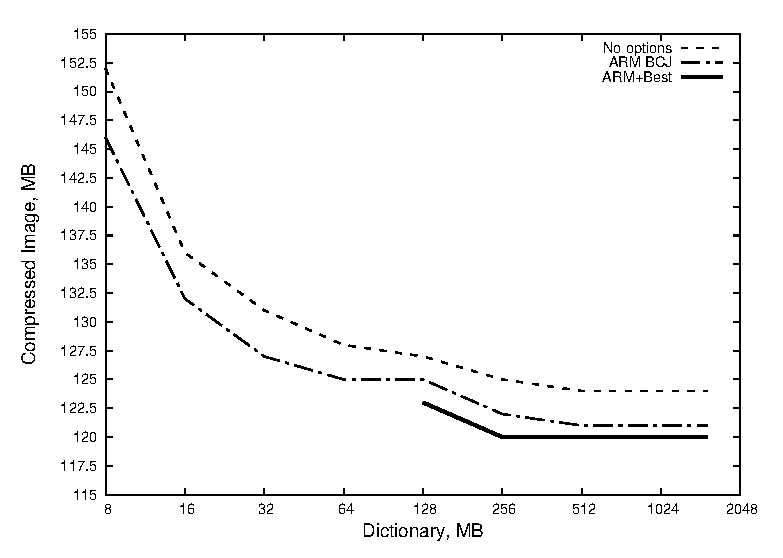
\includegraphics[width=3in]{trik.eps}
	\caption{Improvement in size, TRIK image}
	\label{trik_improvements_figure}
\end{figure}


% Note that the IEEE does not put floats in the very first column
% - or typically anywhere on the first page for that matter. Also,
% in-text middle ("here") positioning is typically not used, but it
% is allowed and encouraged for Computer Society conferences (but
% not Computer Society journals). Most IEEE journals/conferences use
% top floats exclusively. 
% Note that, LaTeX2e, unlike IEEE journals/conferences, places
% footnotes above bottom floats. This can be corrected via the
% \fnbelowfloat command of the stfloats package.

After experimenting with the TRIK image, we tried to see what advanced options will give the best compression ratio when compressing Raspbian image. Remarkably, the \textbf{\textit{lc, lp, pb}} values that worked out for the TRIK image are also the best for the Raspbian image. The whole setup looks like this:
% * <Максим Голов> 15:09:00 17 Mar 2016 UTC+0300:
% 1) After experimenting with the TRIK image, we tried to see what advanced options will give the best compression ratio for Raspbian image. 
% 2) Remarkably, the \textbf{\textit{lc, lp, pb}} values that worked out for the TRIK image are also the best for the Raspbian image.
\begin{itemize}
\item lc=1
\item lp=2
\item pb=2
\item nice=273
\item depth=1024
\end{itemize}

It was already noted that compressing Raspbian is done well with \textbf{\textit{nice}} value equal to 273, while TRIK image gives better results on \textbf{\textit{nice}} equal to 192, which, in theory, is weird, because bigger match length should result in better compression ratio. But we must say that going with \textbf{\textit{nice}} value of 273 produces only 0,2 MB bigger archive than with \textbf{\textit{nice}} of 192 when compressing TRIK firmware image, so one may not be bothered by it and just set \textbf{\textit{nice}} to 273. 
% * <Максим Голов> 15:13:31 17 Mar 2016 UTC+0300:
% 1) It was already noted that Raspbian works well with \textbf{\textit{nice}} value of 273, while the TRIK image gives better results on \textbf{\textit{nice}} of 192, which, in theory, is weird, because bigger match length should result in better compression ratio. 
% 2) But we must say that going with \textbf{\textit{nice}} value of 273 produces only 0,2 MB bigger archive than with \textbf{\textit{nice}} of 192 when compressing TRIK firmware image, so one may not be bothered by it and just set \textbf{\textit{nice}} to 273.

Table \ref{raspbian_improvements_table} and Figure \ref{raspbian_improvements_figure} show improvement in compressing the Raspbian image, relative to standard XZ 9 preset setup:
% * <Максим Голов> 15:17:35 17 Mar 2016 UTC+0300:
% 1) Table \ref{raspbian_improvements_table} and Figure shows improvement in compressing the Raspbian image, compared to basic xz -9 setup:
% 
% Рисунок без номера и не привязан + капс на XZ
% ^ <Максим Голов> 15:19:10 17 Mar 2016 UTC+0300:
% и в пдф что ты скидывал после этого идет строчка
% "which makes it a good preset to try on the ARM-based
% firmware"
% тут я её найти не могу, но проверь все равно
% наверное она к тому абзацу, что ты ещё пишешь

\begin{table}[h]
\renewcommand{\arraystretch}{1.5}
% if using array.sty, it might be a good idea to tweak the value of
% \extrarowheight as needed to properly center the text within the cells
\caption{Improvements in compressing Raspbian image}
\label{raspbian_improvements_table}
\centering
\begin{tabular}{| l *{3}{| c } |}
    \hline
    Dictionary & Default & ARM & Best + ARM \\
    \hline
    128 & 0,75 & 2,31 & 2,81 \\
    256 & 1,06 & 2,61 & 3,05 \\
    512 & 1,52 & 3,06 & 3,49 \\ 
    1024 & 2,01 & 3,54 & 3,97 \\ 
    1536 & 2,92 & 4,43 & 4,87 \\
\hline
\end{tabular}
\end{table}

\begin{figure}[h]
    \centering
	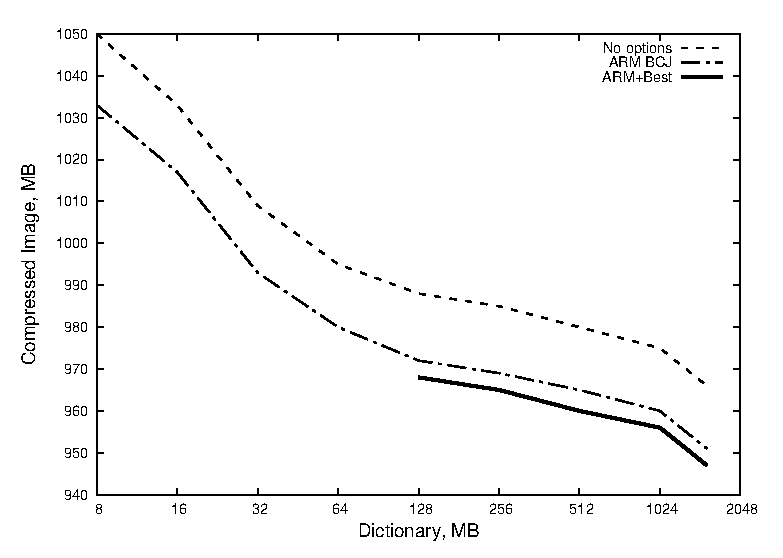
\includegraphics[width=3in]{raspbian.eps}
	\caption{Improvement in size, Raspbian image}
	\label{raspbian_improvements_figure}
\end{figure}

Table \ref{trik_improvements_table}, table \ref{raspbian_improvements_table} as well as figure \ref{trik_improvements_figure} and figure \ref{raspbian_improvements_figure} show that it is definitely worth to try applying the preset that worked out that well for both TRIK and Raspbian to compression of any ARM-based image.
% * <Роман Белков> 13:35:58 17 Mar 2016 UTC+0300:
% label preset; what preset is `this` preset

At last, we decided to see what preset is most useful when compressing MinnowBoard Max firmware image. It is fascinating, because MinnowBoard Max has x86 architecture and before this moment we only paid attention to firmware images for ARM-based controllers.
The best setup for MinnowBoard looks like this: 
\begin{itemize}
\item lc=4
\item lp=0
\item pb=2
\item nice=192
\item depth=1024
\end{itemize}

\begin{table}[h]
\renewcommand{\arraystretch}{1.5}
% if using array.sty, it might be a good idea to tweak the value of
% \extrarowheight as needed to properly center the text within the cells
\caption{Improvements in compressing MinnowBoard image}
\label{minnowboard_improvements_table}
\centering
\begin{tabular}{| l *{3}{| c } |}
    \hline
    Dictionary & Default & X86 & Best + X86 \\
    \hline
    128 & 0,97 & 4,32 & 4,57 \\
    256 & 2,09 & 5,41 & 5,62 \\
    512 & 4,16 & 7,36 & 7,56 \\ 
    1024 & 5,06 & 8,10 & 8,35 \\ 
    1536 & 5,08 & 8,20 & 8,43 \\
\hline
\end{tabular}
\end{table}

\begin{figure}[h]
    \centering
	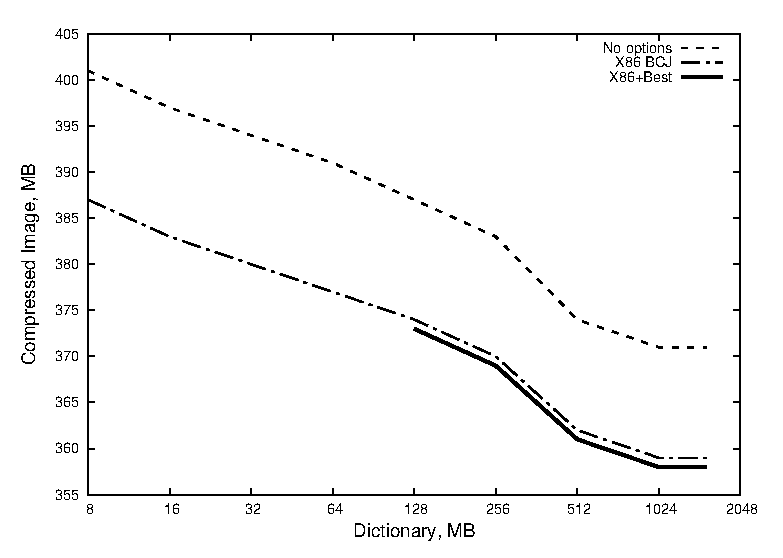
\includegraphics[width=3in]{minnowboard.eps}
	\caption{Improvement in size, Minnowboard image}
	\label{minnowboard_improvements_figure}
\end{figure}

As we have already established \textbf{\textit{nice}} value of 192 works out better than 273. In the case of the TRIK image, the difference was so small that one may set \textbf{\textit{nice}} to 273. It is worth mentioning that tweaking additional options does not produce notable decrease in compression ratio in case of MinnowBoard image, since difference is about 1.5 MB between X86 and Best + X86 setups. However, time increase is not that big (about 45 sec), so we still highly recommend to use best option, because it can provide better result in case of compressing bigger x86 images.
% * <Максим Голов> 21:23:30 18 Mar 2016 UTC+0300:
% 1) As we have already established \textbf{\textit{nice}} value of 192 works out better than 273.
% 2) In the case of the TRIK image, the difference was so small that one may set \textbf{\textit{nice}} to 273.

Now, we are ready to make an overall verdict of what happened. 
% * <Роман Белков> 14:19:18 18 Mar 2016 UTC+0300:
% revise

\begin{table}[h]
\renewcommand{\arraystretch}{1.5}
% if using array.sty, it might be a good idea to tweak the value of
% \extrarowheight as needed to properly center the text within the cells
\caption{Overall improvements}
\label{overall_table}
\centering
\begin{tabular}{| l *{4}{| c } |}
    \hline
    Image & TRIK & Raspbian & RPi Win10 & MB Win10 \\
    \hline
    Before, MB & 158 & 1471 & 500 & 525 \\
% * <Максим Голов> 15:20:52 17 Mar 2016 UTC+0300:
% Лучше Before
    After (prod.), MB & 120,9 & 965,2 & 340,3 &  369,2 \\
    After (best), MB & 120,2 & 947,1 & 332,6 & 359,1 \\
% * <Максим Голов> 15:21:00 17 Mar 2016 UTC+0300:
% Лучше After
    \hline
    \hline
    Improvement (prod), \% & 23,48 & 34,17 & 31,94 & 29,52 \\
    Improvement (best), \% & 23,92 & 35,61 & 33,48 & 31,6 \\
% * <Максим Голов> 15:23:11 17 Mar 2016 UTC+0300:
% Тут я не знаю, что лучше
% Но слово Profit убирай из этого документа вообще)
% Если имеешь в виду уменьшение размера файла, то "File size decrease, %", если что-то другое то поясни -- придумаем что-нибудь другое
\hline
\end{tabular}
\end{table}

Table \ref{overall_table} shows the actual sizes of images downloaded by us from distributors (Before), as well as our compression results (After(prod.) \& After(best)) with corresponding improvements over the distributed archives in percent. The difference between production and best results is in the dictionary size. We decided to differentiate results because the archive that was compressed using the bigger dictionary takes up more RAM when decompression is in process. In fact, RAM for decompression = dictionary size + 1MB. Therefore, we propose that for production dictionary should be set to 256MB, while for best compression ratio dictionary should be set to 1536MB.
% * <Максим Голов> 21:26:46 18 Mar 2016 UTC+0300:
% 1) The difference between production and best results is in the dictionary size.
% 2) We decided to differentiate results because the archive that was compressed using the bigger dictionary takes up more RAM when decompression is in process.

\textbf{Please note}: In Table \ref{overall_table} compression sizes and improvement in percent for Raspberry Pi Windows 10 IoT image  are given in ARM-Thumb configuration because authors did not have time and resources for experimenting with advanced options of this image.
    
\section{Further Work}

\subsection{Multi-Threaded Compression}
Apart from our experiment that is focused on decreasing compression ratio using only one thread, there can be an experiment covering multi-threaded compression in a similar fashion. We did not cover multi-threaded compression since XZ currently utilizes poor compression algorithm that splits data in blocks and compresses them independently, which results in bigger compressed archive and significantly bigger RAM consumption \cite{link:xz-mt}. Overview of current algorithm and results of multi-threaded compression as well as implementation of possible optimizations or new algorithms would be very helpful.
% * <Максим Голов> 21:31:28 18 Mar 2016 UTC+0300:
% 1) We did not cover multi-threaded compression since XZ currently utilizes a compression algorithm that splits data in blocks and compresses them independently, which results in bigger compressed archive and significantly bigger RAM consumption \cite{link:xz-mt}. 
% 
% тут я убрал "utterly bad" потому что это слишком жестко, и обычно свои методы так не поливают. но на твоё усмотрение 
% 
% 2) Overview of the current algorithm and results of multi-threaded compression as well as the implementation of possible optimizations or new algorithms would be very helpful.

\subsection{Independent compression by data types}
As it was already mentioned in Section \ref{sec:experiment} Subsection \ref{subsec:bcj}, the possible way to decrease compression ratio is to compress different data types with different options of XZ instead of blindly applying BCJ filter on the whole image.
% * <Максим Голов> 21:34:04 18 Mar 2016 UTC+0300:
% 1) As it was already mentioned in Section \ref{sec:experiment} Subsection \ref{subsec:bcj}, the possible way to decrease compression ratio is to compress different data types with different options of XZ instead of blindly applying BCJ filter on the whole image.
% 
% Тут точно "to decrease compression ratio" ? ты же увеличиваешь его вроде. но я хз
% ^ <Роман Белков> 21:40:51 18 Mar 2016 UTC+0300:
% да, всё ок тут

\section{Conclusion}
As a result, authors were able to produce the experiment, which can be repeated \cite{link:xz-github} and that shows that application of a proper tool with accurately tuned options has a strong positive impact on compression thus saving distributors and users approximately 30\% of disk space. Some may say that it is not important to use data compression today with all the modern improvements in data storage and networks, but these savings allow to lessen server maintenance costs and decrease download time for user. Although our temptation to say that everyone should use the very best options described previously is high, that would be misleading since best compression ratio is achieved using dictionary of 1536MB, and it is wrong to rely on fact that every user has 1,5GB RAM for decompression. That is why we suggest using 256MB dictionary for production image that would be widely used and using 1536MB dictionary for something not so widely-oriented, e.g. distributing night builds or technical preview builds, because these images are made for narrow set of enthusiasts and usually these people have more technical opportunities thus allowing them to handle archives that require more RAM to be decompressed.
% * <Максим Голов> 21:44:08 18 Mar 2016 UTC+0300:
% 1) In conclusion, authors were able to produce the experiment, which can be repeated and that shows that application of a proper tool with accurately tuned options has a strong positive impact on compression thus saving distributors and users approximately 30\% of disk space.
% 
% тут ссылку пятую верни -- я убрал её
% 
% 2) useless убери, это тоже не очень. оставь только misleading

% use section* for acknowledgment
\section*{Acknowledgment}


The authors would like to thank Maxim Golov and Dmitry Lesnikov for their constructive reviews and helpful advice.
% * <Максим Голов> 21:44:18 18 Mar 2016 UTC+0300:
% наааайс


% trigger a \newpage just before the given reference
% number - used to balance the columns on the last page
% adjust value as needed - may need to be readjusted if
% the document is modified later
%\IEEEtriggeratref{8}
% The "triggered" command can be changed if desired:
%\IEEEtriggercmd{\enlargethispage{-5in}}

% references section
\nocite{*}

\printbibliography
\end{document}


